\PassOptionsToPackage{svgnames}{xcolor}
\documentclass[12pt]{article}



\usepackage[margin=1in]{geometry}  
\usepackage{graphicx}             
\usepackage{amsmath}              
\usepackage{amsfonts}              
\usepackage{framed}               
\usepackage{amssymb} 
\usepackage{array}
\usepackage{amsthm}
\usepackage[nottoc]{tocbibind}
\usepackage{bm}
\usepackage{enumitem}


  \newcommand\norm[1]{\left\lVert#1\right\rVert}
\setlength{\parindent}{0cm}
\setlength{\parskip}{0em}
\newcommand{\Lim}[1]{\raisebox{0.5ex}{\scalebox{0.8}{$\displaystyle \lim_{#1}\;$}}}
\newtheorem{definition}{Definition}[section]
\newtheorem{theorem}{Theorem}[section]
\newtheorem{notation}{Notation}[section]
\theoremstyle{definition}
\DeclareMathOperator{\arcsec}{arcsec}
\DeclareMathOperator{\arccot}{arccot}
\DeclareMathOperator{\arccsc}{arccsc}
\DeclareMathOperator{\PV}{PV}
\DeclareMathOperator{\TV}{TV}
\DeclareMathOperator{\diff}{d}
\DeclareMathOperator{\expec}{E}
\DeclareMathOperator{\var}{Var}
\DeclareMathOperator{\cov}{Cov}
\DeclareMathOperator{\CE}{CE}
\DeclareMathOperator{\RP}{RP}
\newcommand\cf[1]{\mathbf{#1}}
\setcounter{tocdepth}{1}
\setcounter{section}{0}
\begin{document}

\title{Revision notes - MA4264}
\author{Ma Hongqiang}
\maketitle
\tableofcontents

\clearpage
%\twocolumn
\section{Static Game of Complete Information}
\subsection{Pure Strategies}
\begin{definition}[Normal Form Representation]
\hfill\\\normalfont
The normal-form representation of an $n$-player game specifies the players'
\begin{itemize}
  \item \textbf{Strategy space} $S_1,\ldots, S_n$, and 
  \item their \textbf{payoff functions} $u_1, \ldots, u_n$, where $u_i: S_1\times \cdots\times S_n \to \mathbb{R}$.
\end{itemize}
We denote this game by $G=\{S_1,\ldots, S_n; u_1,\ldots, u_n\}$.\\
Let $(s_1,\ldots, s_n)$ be a combination of strategies, one for each player. Then $u_i(s_1,\ldots, s_n)$ is the payoff to player $i$ if for each $j=1,\ldots, n$, player $j$ chooses strategy $s_j$.
\end{definition}
\begin{definition}[Strictly Dominated]
\hfill\\\normalfont In a normal-form game $G=\{S_1,\ldots, S_n; u_1,\ldots, u_n\}$, let $s_i', s_i''\in S_i$. Strategy $s_i'$ is strictly dominated by strategy $s_i''$ if 
\[
u_i(s_i', s_{-i})<u_i(s_i'', s_{-i})\;\;\;\forall s_{-i}\in S_{-i}
\]
i.e., for each feasible combination of the other players' strategies, player $i$'s payoff from playing $s_i'$ is \textbf{strictly} less than the payoff from playing $s_i''$.
\end{definition}
Since rational players do not play strictly dominated strategies, we can eliminate these strictly dominated strategies iteratively, so as to reduce the dimension of $S_i, i=1,\ldots, n$, without removing the best response.
\begin{definition}[Best response]
\hfill\\\normalfont In the $n$-player normal-form game $G=\{S_1,\ldots, S_n; u_1,\ldots, u_n\}$, the \textbf{best response} for player $i$ to a combination of other player's strategies $s_{-i}\in S_{-i}$ is
\[
R_i(s_{-i})L=\arg\max_{s_i\in S_i}u_i(s_i, s_{-i})
\]
i.e., $R_i(s_{-i})$ is the \textit{set of best responses} by player $i$ to the other player's strategies $s_{-i}$.
\end{definition}
\textbf{Remark}: $R_i(s_{-i})\subset S_i$ can be an empty set, a singleton, or a finite or infinite set.
\begin{definition}[Nash Equilibrium]
\hfill\\\normalfont In the $n$-player normal-form game $G=\{S_1,\ldots, S_n; u_1,\ldots, u_n\}$, the strategies $(s_i^\ast, \ldots, s_n^\ast)$ is called a \textbf{Nash Equilibrium} if
\[
s_i^\ast \in R_i(s_{-i}^\ast) \;\;\;\forall i=1,\ldots, n
\]
equivalently, 
\[
u_i(s_i^\ast, s_{-i}^\ast) = \max_{s_i\in S_i} u_i(s_i, s_{-i}^\ast)\;\;\;\forall i=1,\ldots, n
\]
In other words, no player has incentive to deviate from Nash Equilibrium.
\end{definition}
To find a Nash Equilibrium in 2 player game, we can use graph. Let $G(R_i)$ denote the graph of $R_i$ defined by
\[
G(R_i)=\{(s_i, s_{-i})\mid s_i\in R_i(s_{-i}), s_{-i}\in S_{-i}\}
\]
Then $(s_i^\ast, \ldots, s_n^\ast)\in \cap_{i=1}^n G(R_i)$ if and only if it is in a Nash Equilibrium.\\
Specifically, in a 2-person game, we can compute the graph $R_1(s_2)$ and $R_2(s_1)$ and find the intersection.\\
If the game can be represented via a bimatrix, we can use the underline to denote the other player's best payoff to current player's strategy; do this for the 2 players and the cell with both underlined will be the best strategy.
\begin{theorem}[Relation between Nash Equilibrium and IESDS]
\hfill\\\normalfont If the strategies $(s_1^\ast, \ldots, s_n^\ast)$ are a Nash equilibrium in an $n$-player normal-form game $G=\{S_1,\ldots, S_n; u_1,\ldots, u_n\}$, then each $s_i^\ast$ cannot be eliminated in iterated elimination of strictly dominated strategies.
\end{theorem}
This implies: $\{\text{Nash Equilibria}\}\subseteq \{\text{Outcomes of IESDS}\}$.
\begin{theorem}
\hfill\\\normalfont In the $n$-player normal-form game $G=\{S_1,\ldots, S_n; u_1,\ldots, u_n\}$ where $S_1,\ldots, S_n$ are \textit{finite} sets, if IESDS eliminates all but the strategy $(s_1^\ast, \ldots, s_n^\ast)$, then these strategies are unique Nash equilibrium of the game.
\end{theorem}
In general, to compute Nash Equilibrium, find out expression $\pi_i(s_i, s_j)$ (usually in the form of piecewise functions), and take maximum to get a equation $s_i(s_j)$. Similarly, compute $\pi_j$ and get a equation $s_j(s_i)$. Find all intersections.
\subsection{Mixed Strategies}
\begin{definition}[Mixed Strategy]
\hfill\\\normalfont In the normal-form game $G=\{S_1,\ldots, S_n; u_1,\ldots, u_n\}$. Suppose $S_i=\{s_{i1}, \ldots, s_{iK}\}$. Then
\begin{itemize}
  \item Each strategy $s_{ik}$ in $S_i$is called a pure strategy for player $i$.
  \item A mixed strategy for player $i$ is a probability distribution $p_i(p_{i1}, \ldots, p_{iK})$, where $\sum_{k=1}^K p_{ik}=1$ and $p_{ik}\geq 0$.
\end{itemize}
We define the expected payoff for player $1$ to play mixed strategy $p_1:=(p_{11}, \ldots, p_{1J}$ is
\[
v_1(p_1,p_2)=\sum_{j=1}^J \sum_{k=1}^K p_{1j}p_{2k}u_1(s_{1j}, s_{2k})
\]
\end{definition}
\begin{definition}[Nash Equilibrium]
\hfill\\\normalfont In the two-player normal-form game $G=\{S_1,S_2; u_1,u_2\}$, the mixed strategies $(p_1^\ast, p_2^\ast)$ are a \textbf{Nash equilibrium} if each player's mixed strategy is a best response to the other player's mixed strategy, i.e.,
\[
v_1(p_1^\ast, p_2^\ast)\geq v_1(p_1, p_2^\ast)
\]
and 
\[
v_2(p_1^\ast, p_2^\ast)\geq v_2(p_1^\ast, p_2)
\]
for all probability distribution $p_1, p_2$ on $S_1, S_2$.
\end{definition}
Since it is completely known to us the value of $u_{1,2}(s_{1j}, s_{2k})$, the mixed strategy Nash Equilibrium only concerns solving the probability distribution. In a simplified setting where each player has only 2 strategies, let $p_1:=(r, 1-r)$ and $p_2=(q, 1-q)$, then 
\[
v_1(p_1, p_2)=rv_1(s_{11}, p_2)+(1-r)v_1(s_{12}, p_2)
\]
As you can see, $r$ here is dependent on $q$. So we can solve $r^\ast(q)$ by maximising the above equation. Specifically, we can have
\[
r^\ast(q)=\begin{cases}
1, &\text{ if }v_1(s_{11}, p_2)>v_1(s_{12}, p_2)\\
0, &\text{ if }v_1(s_{11}, p_2)<v_1(s_{12}, p_2)\\
[0,1], &\text{ if }v_1(s_{11}, p_2)=v_1(s_{12}, p_2)
\end{cases}
\]
And this is also true for $q^\ast(r)$. Then find intersections.
\begin{theorem}[Strategies eliminated by IESDS]
\hfill\\\normalfont If a pure strategy $s_{kj}\in S_{kj}$ is eliminated by IESDS, then this strategy will be played with zero probability $p_{kj}=0$, in any mixed strategy Nash Equilibrium. If there are only 2 strategies left for each player, then we can use the approach discussed before.
\end{theorem}
\begin{theorem}[Existence Theorem on Nash Equilibrium]
\hfill\\\normalfont In the $n$-player normal-form game $G=\{S_1,\ldots, S_n; u_1,\ldots, u_n\}$, if $n$ is \textit{finite} and $S_i$ is \textit{finite} for every $i$, then there eixsts at least one Nash equilibrium, possibly involving mixed strategies.
\end{theorem}
\clearpage
\section{Dynamic Games on Complete Information}
\begin{definition}[Dynamic Game of Complete and Perfect Information]
\hfill\\\normalfont A dynamic game of complete and perfect information is a game where
\begin{itemize}
  \item Players move in sequence, 
  \item (Perfect Information) All previous moves are observed before next move is chosen,
  \item (Complete Information): Payoffs are common knowledge
\end{itemize}
\end{definition}
Such games can be represented by a game tree.\\
\begin{figure}[h]
\centering
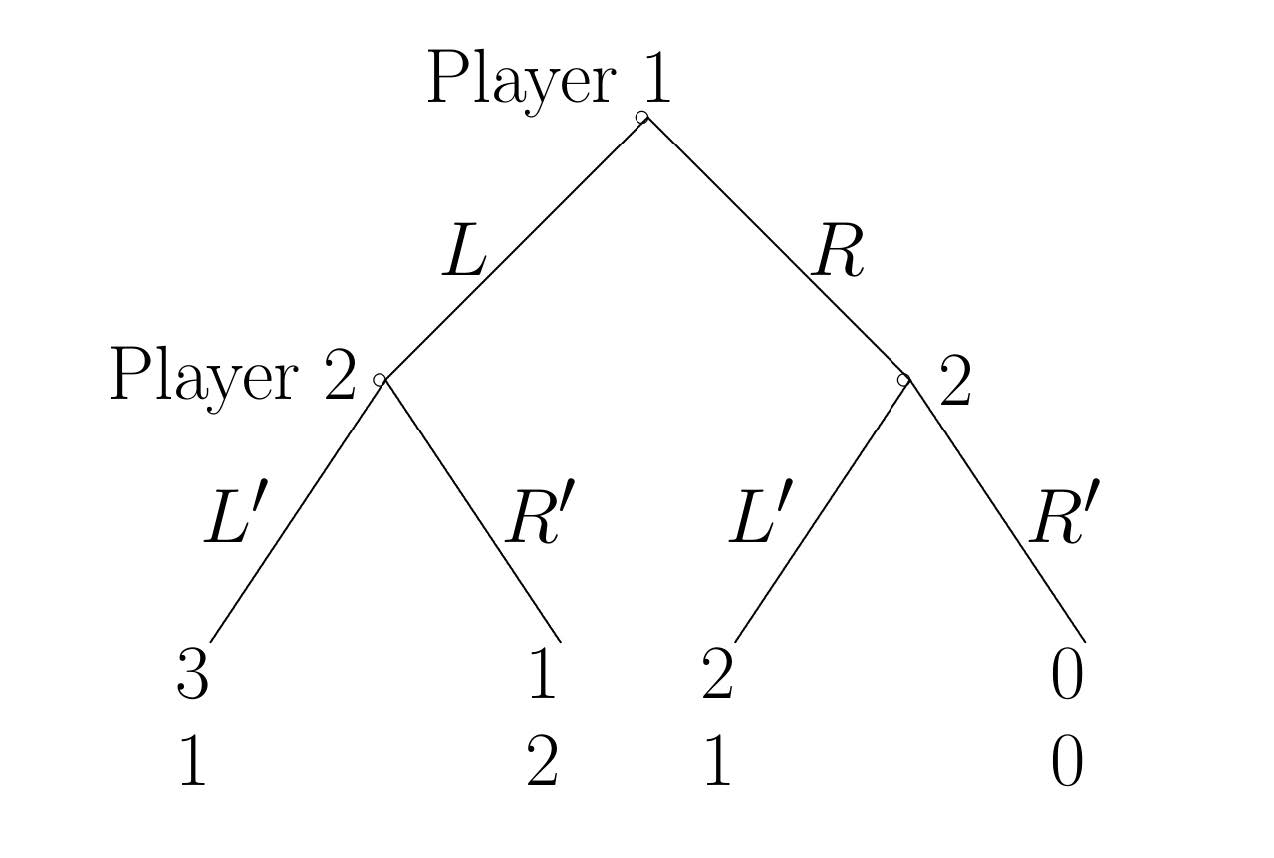
\includegraphics[width=0.7\textwidth]{2-1.jpg}
\end{figure}
In this chapter, we will see games with perfect, and imperfect information in sequence.
\begin{definition}[Backward Induction]
\hfill\\\normalfont The steps are as follow:
\begin{enumerate}
  \item At the second stage, player 2 observes the action chosen by player 1 at the first stage, say $a_1$, and then chooses an action by solving 
  \[
\arg \max_{a_2\in A_2} u_2(a_1, a_2)
  \]
  Assume this optimization problem has a unique solution, denoted by $R_2(a_1)$. This will be the best response.
  \item Player 1 will then solve $\max_{a_1\in A_1}u_1(a_1, R_2(a_1))$.\\
  Assume it has a unique solution $a_1^\ast$, we call $(a_1^\ast, R_2(a_1^\ast))$ the backwards-induction outcome of the game.
\end{enumerate}
\end{definition}
\subsection{Two Stage Games of Complete, Imperfect Information}
\begin{definition}[Subgame Perfect Outcome]
\hfill\\\normalfont 
Let players 1 and 2 simultaneously choose actions $a_1$ and $a_2$ from the feasible set $A_1, A_2$.\\
Let players 3 and 4 observe the outcome of the first stage $(a_1,a_2)$ and then simultaneously choose action $a_3, a_4$ from the feasible sets $A_3, A_4$ respectively.\\
Payoffs are $u_i(a_1,a_2,a_3,a_4)$ for $i=1,2,3,4$.\\
For each given $(a_1, a_2)$, player 3 and 4 try to find Nash equilibrium in stage 2. Assume the second-stage game has a unique Nash Equilibrium $(a_3(a_1, a_2), a_4(a_1,a_2))$, then player 1 and player 2 play a simultaneous-move game with payoffs $u_i(a_1,a_2,a_3(a_1,a_2), a_4(a_1,a_2))$. Suppose $(a_1^\ast, a_2^\ast)$ is the Nash equilibrium of the simultaneous-move game, then
\[
(a_1^\ast, a_2^\ast, a_3(a_1^\ast, a_2^\ast), a_4(a_1^\ast, a_2^\ast))
\]
is the \textbf{subgame-perfect} outcome of the 2-stage game.
\end{definition}
\begin{definition}[Extensive Form Representation]
\hfill\\\normalfont The \textbf{extensive form} representation of a game specifies
\begin{itemize}
  \item The players in teh game
  \item \begin{itemize}
  \item When each player has the move
  \item What each player can do at each move
  \item What each player knows at each of his or her move
  \item The payoff received by each player for each combinations of moves that could be chosen by the players
  \end{itemize}
\end{itemize}
\end{definition}
\begin{definition}[Information Set]
\hfill\\\normalfont An \textbf{information set} for a player is a collection of decision nodes satisfying:
\begin{itemize}
  \item The player needs to move at every node in the information set
  \item When the play of the game reached a node in the information set, the player with the move does not know which node in the set has been reached.
\end{itemize}
The second point impliees the player must have the \textbf{same set} of feasible actions at each decision node in an information set.
\end{definition}
A game is said to have \textbf{imperfect information} if some of its information sets are \textit{non-singletons}.\\
In an extensive-form game, a collection of decision nodes, which constitutes an information set, is connected by a dotted line.
\begin{definition}[Strategy]
\hfill\\\normalfont A \textbf{strategy} for a player is a \textbf{complete plan of actions}.\\
It specifies a feasible action for the player in every contingency in which the player might be called on to act. 
\end{definition}
\begin{definition}[Payoffs]
\hfill\\\normalfont In the extensive-form representation, payoffs are given for \textbf{each sequence of actions}, namely
\[
u_i(a_1,\ldots, a_m), \;\;\;i=1,\ldots, n
\]
where $a_1,\ldots, a_m$ are a sequence of actions.\\
Let $s=(s_1,\ldots, s_n)$ be a combination of strategies of $n$ players and $(a_1(s), \ldots, a_m(s))$ be the sequence of actions specified by $s(s_1,\ldots, s_n)$. Then the payoff received by playing $s=(s_1,\ldots, s_n)$ is
\[
\tilde{u}(s)=u(a_1(s), \ldots, a_m(s))
\]
where $s$ on LHS is strategy while the parameters in the RHS are actions taken.
\end{definition}
\begin{definition}[Normal Form and Nash Equilibrium]
The normal form of dynamic game specifies payoffs for each combination of \textbf{strategies}. Nash Equilibrium is obtained from teh normal-form representation.
\end{definition}
Remark: The Nash Equilibrium for dynamic games concerns about players' respective best \textbf{strategies}.\\
In general, we are interested in finding the Nash Equilibrium $(s_1, s_2)$ where $s_1\in A_1$ and $s_2=f:A_1\to A_2$. This means
\begin{itemize}
  \item Player 1 is interested in finding $\arg\max_{s_1}\tilde{u}_1(a_1=s_1, s_2^\ast)$
  \item Player 2 is interested in finding $\arg\max_{s_2}\tilde{u}_2(a_1, s_2)$ for each $a_1 \in A_1$
\end{itemize}
Here, although $R_2$ gives an $\arg\max$ of whatever player 1 plays, player 2 may \textit{not} follow this strategy.
\begin{theorem}\normalfont $(a_1^\ast, R_2)$ is a Nash equilibrium.
\end{theorem}
However, apart from $a_1^\ast$, there exists other Nash Equilibriums where player 1 not necessarily playing $a_1^\ast$.
\begin{definition}[Subgame Perfect Nash Equilibrium]
\hfill\\\normalfont A \textbf{subgame} in an extensive-form game
\begin{itemize}
  \item begins at a decision node $n$ that is a singleton information set (but is not the game's first decision node)
  \item includes all the decision and terminal nodes following node $n$ in teh game tree (but no nodes that do not follow $n$)
  \item does not cut any information sets (i.e., if a decision node $n'$ follows $n$ in the game tree, then all other nodes in the information set containing $n'$ must also follow $n$, and so must be included in teh subgame)
\end{itemize}
A Nash Equilibrium is \textbf{subgame-perfect} if the players' strategies constitute a Nash Equilibrium in every subgame.
\end{definition}
It can be shown that any finite dynamic game of complete information has a subgame-perfect Nash Equilibrium (which can be in mixed strategies).
\subsection{Infinitely Repeated Games}
Let $\pi_t$ be the payoff in stage $t$. Given a discount factor $\delta\in (0,1)$, the \textbf{present value} of sequence of payoff $\{\pi_1,\pi_2,\ldots\}$ is
\[
\pi_1+\delta\pi_2+\cdots = \sum_{t=1}^\infty \delta^{t-1} \pi_t
\]
Here the period 1 is un-discounted.
\begin{definition}[Infinitely Repeated Games]
\hfill\\\normalfont In the first stage, the player play the stage game $G$, and receive payoff $\pi_{1,1} and \pi_{2,1}$.\\
The game is repeated infinitely. In the $t$th stage, the players observe the actions chosen in the preceding $(t-1)$ stages, and then play $G$ to receive $(\pi_{1,t}, \pi_{2,t})$\\
The payoff of infinitely repeated game is the \textbf{presetn value} of sequence of payoffs:
\[
(\sum_{t=1}^\infty \delta^{t-1}\pi_{1,t}, \sum_{t=1}^\infty \delta^{t-1}\pi_{2,t})
\]
Playing the stage game $G$ does not mean having to play an equilibrium of $G$.\\
Denote by $A_{it}$ the action space of player $i$ in stage $t$. We have $A_t:=A_{1t}\times A_{2t}$.\\
A strategy by player $i$ is of the form $\{a_{i1}, a_{i2},\ldots\}$ where $a_{it}:A_1\times\cdots\times A_{t-1}\to A_{it}$.\\
The payoff received at stage $t$ is $\pi_{it}=u_i(a_{it}, a_{jt})$.
\end{definition}
Here, the non-cooperative strategy in Infinite Prisoner Dilemma is a Nash Equilibrium, whereas \textit{trigger strategy} is a Nash Equilibrium if and only if $\delta\geq \frac{1}{4}$. A trigger strategy chooses cooperation until being betrayed.
\begin{theorem}\normalfont Trigger strategy Nash Equilibrium($\delta\geq 1/4$) is subgame perfect.\end{theorem}
\clearpage
\section{Static games of incomplete information}
Games of \textbf{incomplete information} are also called \textbf{Bayesian games}. In a game of \textit{incomplete} information, at least one player is uncertain about another player's payoff function.\\
If there are uncertainty, we will maximise the \textit{expected} profit.\\
In general, let player $i$'s possible payoff functions by $u_i(a_1,\ldots, a_n; t_i)$ where $t_i\in T_i$ is the \textbf{type} of player $i$.\\
Let $t_{-i}$ be the types of other players and $T_{-i}$ the set of all the $t_{-i}$.\\
Player $i$ knows his own type, but \textit{only} knows probability distribution $P_i(t_{-i}\mid t_i)$ on $T_{-i}$, a belief about other player's types, given $i$'s knowledge of his own $t_i$.
\begin{definition}[Normal-form Representation]
\hfill\\\normalfont The \textbf{normal-form} representation of an $n$-player static Bayesian game specifies
\begin{itemize}
  \item Players' action spaces $A_1,\ldots, A_n$
  \item Player's type spaces $T_1,\ldots, T_n$
  \item their beliefs $P_1,\ldots, P_n$ where $P_i: T_i\to P(T_{-i}\mid T_i)$
  \item their payoff functions $u_1,\ldots, u_n$ where $u_n:\prod_i A_i \times t_i$.
\end{itemize}
We denote the game as $G=\{A_1,\ldots, A_n; T_1,\ldots, T_n; P_1,\ldots, P_n; u_1,\ldots, u_n\}$.\\
The timing is as follows:
\begin{itemize}
  \item Nature draws a type vector $t=(t_1,\ldots, t_n)$
  \item Nature reveals $t_i$ to player $i$ only.
  \item Players simultaneously choose action $a_i\in A_i$
  \item Payoff $u_i(a_1,\ldots, a_n; t_i)$are received
\end{itemize}
Suppose we have a prior probability distribution $P(t): T \to \mathbb{R}$, then the belief $P_i(t_{-i}\mid t_i)$ can be computed by Bayes' rule:
\[
P(t_{-i}\mid t_i) =\frac{P(t_{-i}, t_i)}{P(t_i)}=\frac{P(t_{-i},t_i)}{\sum_{t_{-i};\in T_{-i}}P(t_{-i}', t_i)}
\]
\end{definition}
\begin{definition}[Strategy]
\hfill\\\normalfont In the static Bayesian Game $G$, a \textbf{strategy} for player $i$ is a function $s_i: T_i\to A_i$.\\
For given type $t_i$, $s_i(t_i)$ gives the action. Player $i$'s strategy space $S_i$ is set of all functions from $T_i$ to $A_i$.
\end{definition}
\begin{definition}[Bayesian Nash Equilibrium]
\hfill\\\normalfont In static Bayesian game $G$, the strategies $s^\ast = (s_1^\ast, \ldots, s_n^\ast)$ are a pure-strategy \textbf{Bayesian Nash Equilibrium} if, for each player $i$ and each of $i$'s type $t_i$, $s_i^\ast(t_i)$ solves
\[
\max_{a_i\in A_i} E_{t_i} u_i(a_i, s_{-i}^\ast(t_{-i}); t_i)
\]
where 
\[
E_{t_i} u_i(a_i, s_{-i}^\ast(t_{-i}); t_i) = \sum_{t_{-i}\in T_{-i}} P_i(t_{-i}\mid t_i)u_i(a_i, s_{-i}^\ast(t_{-i}); t_i)
\]
\end{definition}
\begin{theorem}\normalfont In a general, finite action space static Bayesian game, a Bayesian Nash equilibrium exists, perhaps in mixed strategies.\end{theorem}
The steps we take to find Nash Equilibrium is 
\begin{itemize}
  \item For each player,
  \begin{itemize}
    \item For each type of games itself has
    \begin{itemize}
      \item Draw tables of payoff, one each for each type of games opponent has
    \end{itemize}
    \item Collate the tables into an expected payoff table of itself playing this type
  \end{itemize}
  \item Collate the tables generated to the best response $R_i: S_i\to S_j$.
  \item Use a table to find out Nash Equilibrium, with rows and columns populated by all possible strategies. This is because, $R$ may map to a set.
\end{itemize}
\begin{definition}[``Nature Select a Game'' Form]
\hfill\\\normalfont Nature selects a game from a set of possible games for each player to play. Some player may know some information about which games/subset of games he is playing.\\
In general, such static Bayesian games are defined by $\{G,P,(T_1,\ldots, T_n)\}$, where
\begin{itemize}
  \item $G$ a set of games, where $g\in G$ specifies players' action spaces $A_i$ and payoffs $u_i(a;g)$ for $a=(a_1,\ldots, a_n), \;i=1,\ldots, n$.
  \item $P$ a probability distribution of $G$
  \item $T_i$ player $i$'s type space, where each $t_i\in T_i$ is a subset of $G$, and type space $T_i$ a partition of $G$.
  \item The players' types are determined by nature. If nature selects $g\in G$, the player will have type $t_j$ where $g\in t_j$.
  \item Define $\sigma_i:G\to T_i$, $\sigma_i(g)=t_i$ if $g\in t_i$. So it maps the games to type.
  \item $(\sigma_1,\ldots, \sigma_n)$ are common knowledge.
\end{itemize}
The games proceeds as such
\begin{itemize}
  \item Nature selects a game
  \item Each player learns its own type, but not others'.
  \item Player act given its type.
\end{itemize}
\end{definition}
To find equilibria, consider a strategy profile $s_{-i}:T_{-i}\to A_{-i}$ of other $n-1$ players,
\begin{itemize}
  \item Let $u_i(a_i,s_{-i}; t_i)$ be the expected payoff received by type $t_i$ of player $i$ if $i$ players $a_i$.
  \item $(s_i^\ast, s_{-i}^\ast)$ is a Bayesian equilibrium if for each $t_i\in T_i$
  \[
u_i(s_i^\ast(t_i), s_{-i}^\ast; t_i) = \max_{a_i\in A_i} u_i(a_i, s_{-i}^\ast; t_i)
  \]
\end{itemize}
\begin{theorem}\normalfont For any type $t_i\in T_i$, and strategy profile $s_{-i}$, 
\[
u_i(a_i,s_{-i}; t_i) =\frac{1}{P(t_i)}\sum_{g\in t_i}P(g)u_i(a_i; s_{-i}(\sigma_{-i}(g));g)
\]
\end{theorem}
Here, we take the following steps to find equilibria:
\begin{itemize}
  \item For each player,
  \begin{itemize}
    \item For each type, compute the expected payoff
    \item Find best response
  \end{itemize}
\end{itemize}
The important tables are the payoff table of each game as well as the formula.
\begin{theorem}[Weakly Dominating Leading Bayesian NE]
\hfill\\\normalfont Let $(s_1^\ast, \ldots, s_n^\ast)$ be strategies in a static Bayesian game. If for any $t_i\in T_i, a_i\in A_i$ and $a_{-i}\in A_{-i}$,
\[
u_i(s_i^\ast(t_i), a_{-i}; t_i) \geq u_i(a_i, a_{-i}; t_i)
\]
(i.e., $s_i^\ast(t_i)$ weakly dominates every $a_i\in A_i$), then $(s_1^\ast, \ldots, s_n^\ast)$ is a Bayesian Nash Equilibrium.
\end{theorem}
\clearpage
\section{Dynamic Games of Incomplete Information}
\subsection{Perfect Bayesian Equilibrium}
\begin{definition}[Perfect Bayesian Equilibrium]
\hfill\\\normalfont A \textbf{perfect Bayesian equilibrium} consists of \textbf{strategies} \textit{and} \textbf{beliefs} satisfying the following requirements:
\begin{itemize}
  \item Given their beliefs, the players' strategies must be \textbf{sequentially rational}. \\That is, at each information set, the action taken by the player with the move (and the player's subsequent strategy) must be optimal, given the player's belief at that information set and the other players' subsequent strategies, (where a ``subsequent strategy'' is a complete plan of action covering every contingency that might arise after the given information set has been reached).
  \item \textbf{Consistency}: At every information set, beliefs are determined by Bayes' rule and the players' strategies, whenever possible.
\end{itemize}
\end{definition}
\textbf{Remark}: The strategy profile in any perfect Bayesian equilibrium is a Nash Equilibrium.
\begin{definition}[Pure Strategy Perfect Bayesian Equilibrium]
\hfill\\\normalfont A \textbf{pure strategy} perfect Bayesian Equilibrium in a signalling game is a pair of strategies and a belief satisfying sequential rationality and consistency.
\end{definition}
\begin{definition}[Sender Receiver Game]
\hfill\\\normalfont In sender receiver game, the nature will choose the type of the game. In each type, there are some actions that the sender can take, and the receiver will act on the actions of the sender but not the type(which is unknown). The payoffs are perfect information to both players.
\end{definition}
For sender-receiver game, the following steps are used to determine perfect bayesian equilibrium.
\begin{itemize}
  \item For each case, determine the Nash Equilibrium(sequentially rational). This can be done by backward induction, or via normal-form representation.
  \item Determine the belief from the case
  \item Check the optimality according to the belief(consistent)
\end{itemize}
\begin{definition}[Worker-Firm]
\hfill\\\normalfont The nature draws the ability of the worker $\{\eta_H, \eta_L\}\in \eta$, and the worker will execute the strategy $S_W:\eta\to \{e_c, e_s\}\in e$, the educational level. The firm will execute the strategy $S_F: e\to w$, the wage.\\
In general, The payoff of the worker is $w-c(\eta_{\cdot}, e_{\cdot})$, whereas the payoff of the firm is $-[y(\eta_{\cdot}, e_{\cdot})-w]^2$, whereas $c$ and $y$ are some functions.
\end{definition}
\begin{theorem}\hfill\\\normalfont Let $c(\eta, e)=c_1(\eta)+c_2(e)$. Assume the worker's payoffs from playing $e_c$ and $e_s$ are different, then there does not exist separating perfect Bayesian equilibrium.\\
The possible Bayesian Equilibria are
\begin{itemize}
  \item $\{(e_c,e_c), (w^\ast(e_c,p), w*\ast(e_s,q)), p=1/2, q\in [0, \bar{q}]\}$
  \item $\{(e_s,e_s), (w^\ast(e_c,p), w*\ast(e_s,q)), p\in [0, \bar{p}], q=1/2\}$
\end{itemize}
where $w^\ast(e_i, r)=ry(\eta_H, e_i)+(1-r)y(\eta_L, e_i)$, $\bar{q}$ the maximum that $\frac{1}{2}B(\eta_H,e_c)+\frac{1}{2}B(\eta_L, e_c)\geq qB(\eta_H, e_s)+(1-q)B(\eta_L, e_s)$ holds; $\bar{p}$ the maximum that $pB(\eta_H,e_c)+(1-p)B(\eta_L, e_c)\leq \frac{1}{2}B(\eta_H, e_s)+\frac{1}{2}B(\eta_L, e_s)$ holds, and $B(\eta_{\cdot}, e_{\cdot})=y(\eta_{\cdot}, e_{\cdot})-c_2(e_{\cdot})$.
\end{theorem}
\clearpage
\section{Cooperative Games}
\begin{definition}[Domination, Pareto Optimal]
\hfill\\\normalfont Let $(u, v)$ and $(u', v')$ be two payoff pairs. We say $(u, v)$ \textbf{dominates} $(u', v')$ if
\[
u\geq u',\;\;\; v\geq v'
\]
Payoff pairs which are not dominated by any other pair are said to be \textbf{Pareto optimal}.
\end{definition}
\begin{definition}[Two-person bargaining game]
\hfill\\\normalfont The pair $\Gamma = (H, d)$ is a \textbf{two-person bargaining game} if
\begin{itemize}
  \item $H\subset \mathbb{R}^2$, the set of payoff pair, is compact(closed and bounded) and convex.
  \item $d\in H$, a threat point
  \item and $H$ contains at least one element $u$, such that $u\gg d$.
\end{itemize}
\end{definition}
\begin{definition}[Nash Bargaining Solution]
\hfill\\\normalfont The Nash bargaining solution is a mapping $f: W\to \mathbb{R}^2$ that associates a unique element $f(H, d)=(f_1(H,d), f_2(H, d))$ with the game $(H, d)\in W$, satisfying the following axioms:
\begin{enumerate}
  \item Feasibility: $f(H,d)\in H$
  \item Individual rationality: $f(H, d)\gg d$ for all $(H, d)\in W$.
  \item $f(H, d)$ is Pareto Optimal.
  \item Invariance under linear transformations:\\
  Let $a_1, a_2>0, b_1, b_2\in \mathbb{R}$ and $(H, d), (H', d')\in W$ where $d_i'=a_id_i+b_i, i=1,2$, and $H'=\{x\in \mathbb{R}^2\mid x_i=a_iy_i+b_i, u=1, 2, y\in H\}$. Then $f_i(H_i', d_i')=a_if_i(H, d)+b_i, i=1,2$.
  \item Symmetry: If $(H, d)\in W$ satisfies $d_1=d_2$ and $(x_1, x_2)\in H$ implies $(x_2, x_1)\in H$, then $f_1(H, d)=f_2(H,d)$.
  \item Independence of irrelevant alternatives:\\
  If $(H, d), (H', d')\in W, d=d', H\subset H'$ and $f(H', d')\in H$, then $f(H, d)=f(H', d')$.
\end{enumerate}
\end{definition}
\begin{theorem}[Solving Nash Bargaining Game]
\hfill\\\normalfont A game $(H, d)\in W$ has a unique Nash solutino $u^\ast=f(H, d)$ satisfying conditions 1 to 6. The solution $u^\ast$ satisfies condition 1 to 6 if and only if
\[
(u_1^\ast - d_1)(u_2^\ast -d_2)>(u_1-d_1)(u_2-d_2)
\]
for all $u\in H$, $u\gg d$ and $u\neq u^\ast$.
\end{theorem}
\begin{definition}[{$n$}=person Cooperative Games]
\hfill\\\normalfont For an $n$-person game with the set of players $N=\{1,2,\ldots, n\}$
\begin{itemize}
  \item any nonempty subset of $N$ is called a \textbf{coalition}
  \item For each coalition $S$, the characteristic function $v$ of the game gives the amount $v(S)$ that the coalition $S$ can be sure of receiving.
  \item The game is denoted by $\Gamma = (N, v)$.
\end{itemize}
\textbf{Assumption}: The characteristic function $v$ satisfies
\begin{enumerate}
  \item $v(\varnothing)=0$
  \item For any \textbf{disjoint} coalitions, $K$ and $L$ contained in $N$, 
  \[
v(K\cup L)\geq v(K)+v(L)
  \]
\end{enumerate}
\end{definition}
\begin{definition}[Imputation]
\hfill\\\normalfont An \textbf{imputation} in the game $(N, v)$ is a payoff vector $x=(x_1,\ldots, x_n)$ satisfying
\begin{enumerate}
  \item $\sum_{i=1}^n x_i=v(N)$ (group rational)
  \item $x_i\geq v(\{i\})$, for all $i\in N$ (individually rational)
\end{enumerate}
\end{definition}
Let $I(N, v)$ denote the set of all imputations of the game $(N, v)$.
\begin{definition}[Dominate]
\hfill\\\normalfont Let $x, y\in I(N, v)$ and let $S$ be a coalition. We say $x$ dominates $y$ via $S$, i.e. $x\succ_S y$, if
\begin{enumerate}
  \item $x_i>y_i$ for all $i\in S$
  \item $\sum_{i\in S} x_i \leq v(S)$
\end{enumerate}
We say $x$ \textbf{dominates} $y$, i.e. $x\succ y$ if there is \textit{any} coalition $S$ such that $x\succ_S y$.
\end{definition}
A dominated imputation is unstable, and we hope to solve to get a undominated imputation.
\begin{definition}[Core]
\hfill\\\normalfont The set of all undominated imputations for a game $(N, v)$ is called the \textbf{core}, denoted by $C(N, v)$.
\end{definition}
\begin{theorem}
\hfill\\\normalfont The core of a game $(N, v)$ is the set of all $n$-vectors $x$, satisfying
\begin{itemize}
  \item $\sum_{i\in S}x_i\geq v(S)$ for all $S\subset N$.
  \item $\sum_{i\in N}x_i = v(N)$
\end{itemize}
\end{theorem}
The core of the game $(N, v)$ is nonempty \textit{if and only if} there exists $x$ satisfying the above theorem, \textit{if and only if} 
\begin{align*}
v(B)\geq &\min_{x\in \mathbb{R}^n} \sum_{i=1}^n x_i\\
&\text{such that }\sum_{i\in S}x_i\geq v(S), \;\;\;\forall S\subset N, S\neq N
\end{align*}
\begin{definition}[Constant Sum Game]
\hfill\\\normalfont A game $(N, v)$ is said to be \textbf{constant sum} if for all $S\subset N$,
\[
v(S)+v(N-S)=v(N)
\]
\end{definition}
\begin{definition}[Essential Game]
\hfill\\\normalfont A game $(N, v)$ is \textbf{essential} if
\[
v(B)> \sum_{i\in N}v(\{i\})
\]
It is \textbf{inessential} otherwise.
\end{definition}
\begin{theorem}\normalfont If $(N, v)$ is inessential, then for any coalition $S$, $v(S)=\sum_{i\in S}v(\{i\})$/
\end{theorem}
\begin{theorem}\normalfont If $(N, v)$ is inessential, then it is constant sum.
\end{theorem}
\begin{theorem}\normalfont If a game $(N, v)$ is constant sum, then its core is either empty or a singleton
\[
\{(v(\{1\}), \ldots,v(\{n\}) )\}
\]
\end{theorem}
\begin{theorem}\normalfont If $(N, v)$ is inessential, then $C(N, v)=\{(v(\{1\}), \ldots,v(\{n\}) )\}$.
\end{theorem}
\begin{theorem}\normalfont If game $(N, v)$ is both essential and constant-sum, then its core is empty.
\end{theorem}
\begin{definition}[Strategically Equivalent]
\hfill\\\normalfont Two games $v, u$ are \textbf{strategically equivalent} if there exist constants $a>0$ and $c_1,\ldots, c_n$ such that for every coalition $S$
\[
u(S)=av(S)+\sum_{i\in S}c_i
\]
\end{definition}
\begin{theorem}\normalfont Suppose that $u$ and $v$ are strategically equivalent. Then
\begin{enumerate}
  \item $u$ is essential(resp. inessential) \textit{if and only if} $v$ is essential(resp. inessential).
  \item $x$ is an imputation for $v$ \textit{if and only if} $ax+c$ is an imputation for $u$, where $c=(c_1,\ldots, c_n)$.
  \item $x\succ_S y$ with respect to $v$ \textit{if and only if} $ax+c\succ_S ay+c$ with respect to $u$.
  \item $x\in C(N, v)$ \textit{if and only if} $ax+c\in C(N, u)$.
\end{enumerate} 
\end{theorem}
\begin{definition}[{$(0,1)$}-reduced form]
\hfill\\\normalfont A characteristic function $v$ is in $(0,1)$\textbf{-reduced form} if
\begin{itemize}
\item $v(\{i\})=0$ for all $i\in N$.
\item $v(N)=1$.
\end{itemize} 
\end{definition}
\begin{theorem}\normalfont Any essential game $(N, v)$ is strategically equivalent to a game $(N, i)$ in $(0,1)$-reduced form.
\end{theorem}
\begin{definition}[Shapley Value]
\hfill\\\normalfont Given $n$-person game $(N, v)$, the Shapley value is a $n$-vector, denoted by $\phi(v)$, satisfying a set of axioms. \\
The $i$th component of $\phi(v)$ can be uniquely determined by
\begin{align*}
\phi_i(v)&=\sum_{S\subseteq N\setminus\{i\}}\frac{s!(n-s-1)!}{n!}[v(S\cup \{i\})-v(S)]\\
&=\frac{1}{n}\sum_{s=0}^{n-1}\frac{1}{\binom{n-1}{s}}\sum_{S\subset N\setminus\{i\}, |S|=s}[v(S\cup\{i\}-v(S))]
\end{align*}
\end{definition}
We can understand $\phi_i(v)$ is the expected contribution of $i$ to coalition. This is because the probability of finding coalition $S$ already there when player $i$ arrives is
\[
\gamma(s)=\frac{s!(n-s-1)!}{n!}
\]
\begin{theorem}\normalfont The Shapley value has the following desirable properties, assuming $v(\varnothing)=0$.
\begin{itemize}
  \item Individual rationality: $\phi_i(v)\geq v(\{i\})$ for every $i\in N$.
  \item Efficiency: The total gain is distributed: $\sum_{i\in N}\phi_i(v)=v(N)$.
  \item Symmetry: If player $i$ and $j$ are such that $v(S\cup\{i\})=v(S\cup\{j\})$ for every coalition $S$ not containing $i$ and $j$, then $\phi_i(v)=\phi_j(v)$.
  \item Additivity: If $v$ and $w$ are characteristic functions, then $\phi(v+w)=\phi(v)+\phi(w)$.
  \item Dummy: If player $i$ is such that $v(S\cup\{i\})=v(S)$ for every $S$ not containing $i$, then $\phi_i(v)=0$.
\end{itemize}
\end{theorem}

\end{document}

